The alpha-beta algorithm is based on the minimax algorithm: it returns the same result, but in a shorter time thanks to the pruning of some sub-trees. Minimax is an algorithm (often implemented in a recursive form as an iterative-deepening DFS) which is used to choose an optimal move for a player assuming that the other player is also playing optimally. Minimax strategy is safe, since it discourages taking any risks. Minimax generates the whole game tree, down to the leaves. Alpha beta pruning has no effect on the evaluation of the terminal states and returns the same result of minimax, i.e. the optimal result.

However, exploring the whole search tree is impossible in most cases, because it is too large and it would require too much resources, both in terms of time and of memory. What is performed instead is a search until a certain depth $d$ (often by means of an iterative-deepening DFS algorithm, as in our case) and the evaluation of the leaves of such trees (the last states reached and not expanded in the search). The evaluations is based on some heuristic functions. If we had a perfect heuristic we would need to perform the search and then the evaluation only one move ahead, but in reality the evaluation functions are always imperfect. The quality of the minimax algorithm, and therefore of the alpha-beta pruning algorithm, depends on its heuristic.  The statement is therefore false: the alpha-beta algorithm i would be optimal only with  a perfect heuristic, and this is not the case. To sum up, the terminal utilities of the final states are replaced by the evaluation function for non-terminal positions. Performing this change in the algorithm makes it non-optimal (but feasible).

Fig. \ref{fig:4} shows an example of a search-space where alpha-beta algorithm evaluates states at $depth=1$ and returns the optimal decision $a1$ according the evaluation (50 is the maximum value among the values computed for the child states), while the algorithm run until the terminal states (no heuristic, no evaluation, just the utility of the terminal states) of the search tree ($depth = 2$) would have returned $a3$: considering an optimal rival, $a1$ eventually returns $utility = 40$, while $a3$ returns a terminal state utility of 42.

\begin{figure}[h]
    \centering
    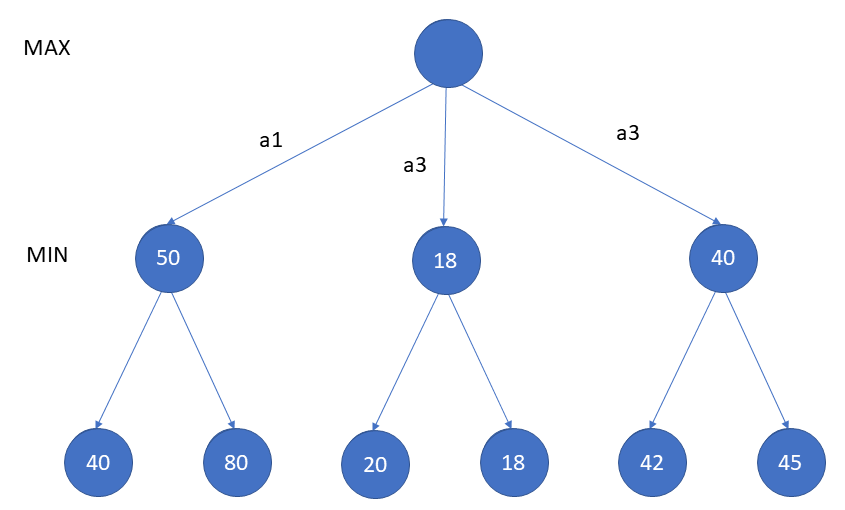
\includegraphics[width=0.6\linewidth]{4}
    \caption{Example of alpha-beta algorithm with heuristic and evaluation at $depth = 1$.}
    \label{fig:4}
\end{figure}